\documentclass[border=0pt]{standalone}
\newcommand{\revlamina}{5}
\providecommand{\revlamina}{1}
% Preámbulo común de las láminas FV (A3 horizontal, 420 x 297 mm)
\usepackage[T1]{fontenc}
\usepackage[utf8]{inputenc}
\usepackage[spanish,es-nodecimaldot]{babel}
\usepackage[scaled=0.92]{helvet}
\renewcommand{\familydefault}{\sfdefault}
\usepackage{tikz}
\usetikzlibrary{arrows.meta,patterns,calc,babel,positioning}
\usepackage{siunitx}
\sisetup{output-decimal-marker={,},mode=text}
\DeclareSIUnit\kWp{kWp}
\DeclareSIUnit\ohm{\ensuremath{\Omega}}

\definecolor{inv1}{RGB}{37,99,180}
\definecolor{inv2}{RGB}{22,128,84}
\definecolor{nfpa}{RGB}{200,30,30}
\definecolor{viento}{RGB}{40,70,200}
\definecolor{sombra}{RGB}{230,130,0}
\definecolor{losa}{RGB}{120,190,200}
\definecolor{dc}{RGB}{225,95,0}
\definecolor{exist}{RGB}{110,110,110}
\definecolor{nuevo}{RGB}{190,20,20}

% Marcador de referencia numerada
\newcommand{\refm}[2]{\node[circle,draw=black,fill=white,line width=0.35pt,inner sep=0pt,minimum size=3.4mm,font=\fontsize{5.5}{6}\selectfont\bfseries] at #1 {#2};}

% Cajetín: \cajetin{lamina}{titulo}{contenido}{escala}{hoja}
\newcommand{\cajetin}[5]{%
  \draw[line width=0.6pt] (250,10) rectangle (410,58);
  \draw[line width=0.3pt] (250,46) -- (410,46);
  \draw[line width=0.3pt] (250,34) -- (410,34);
  \draw[line width=0.3pt] (250,22) -- (410,22);
  \draw[line width=0.3pt] (370,10) -- (370,34);
  \draw[line width=0.3pt] (330,10) -- (330,22);
  \node[anchor=north west,font=\fontsize{6}{7}\selectfont,align=left] at (251.5,57) {\textbf{Instituto Tecnológico de Costa Rica} -- EL-4601 Normalización Técnica para Electrónica\\Proyecto No.~2: Diseño normativo de una instalación solar fotovoltaica};
  \node[anchor=north west,font=\fontsize{6}{7}\selectfont,align=left] at (251.5,45) {\textbf{Proyecto:} Sistema FV 20,88~kWp -- Edificio Centro Académico de Alajuela (TEC)\\\textbf{Propietario:} Universidad Técnica Nacional -- Catastro A-652521-2000};
  \node[anchor=north west,font=\fontsize{6.5}{7.5}\selectfont,align=left,text width=115mm] at (251.5,33) {\textbf{Contenido:} #2\\#3};
  \node[anchor=north west,font=\fontsize{5.5}{6.5}\selectfont,align=left] at (371.5,33) {\textbf{Lámina}};
  \node[font=\fontsize{16}{18}\selectfont\bfseries] at (390,25.5) {#1};
  \node[anchor=north west,font=\fontsize{5.5}{6.5}\selectfont,align=left] at (251.5,21) {\textbf{Elaboró:} Grupo de trabajo EL-4601\\\textbf{Revisó:} \rule{25mm}{0.2pt}\\\textbf{Fecha:} 7/10/2026 \quad \textbf{Rev.:} \revlamina};
  \node[anchor=north west,font=\fontsize{5.5}{6.5}\selectfont,align=left] at (331.5,21) {\textbf{Escala (A3):}\\#4};
  \node[anchor=north west,font=\fontsize{5.5}{6.5}\selectfont,align=left] at (371.5,21) {\textbf{Hoja:}\\#5};
}
% Marco de la lámina
\newcommand{\marco}{%
  \draw[line width=0.2pt,white] (0,0) rectangle (420,297);
  \draw[line width=0.8pt] (10,10) rectangle (410,287);
}

\begin{document}
\begin{tikzpicture}[x=1mm,y=1mm]
\marco
\begin{scope}[shift={(80.00,534.00)},x=20.000mm,y=-20.000mm]
\node[anchor=north west,inner sep=0pt] at (-3.0,12.6) {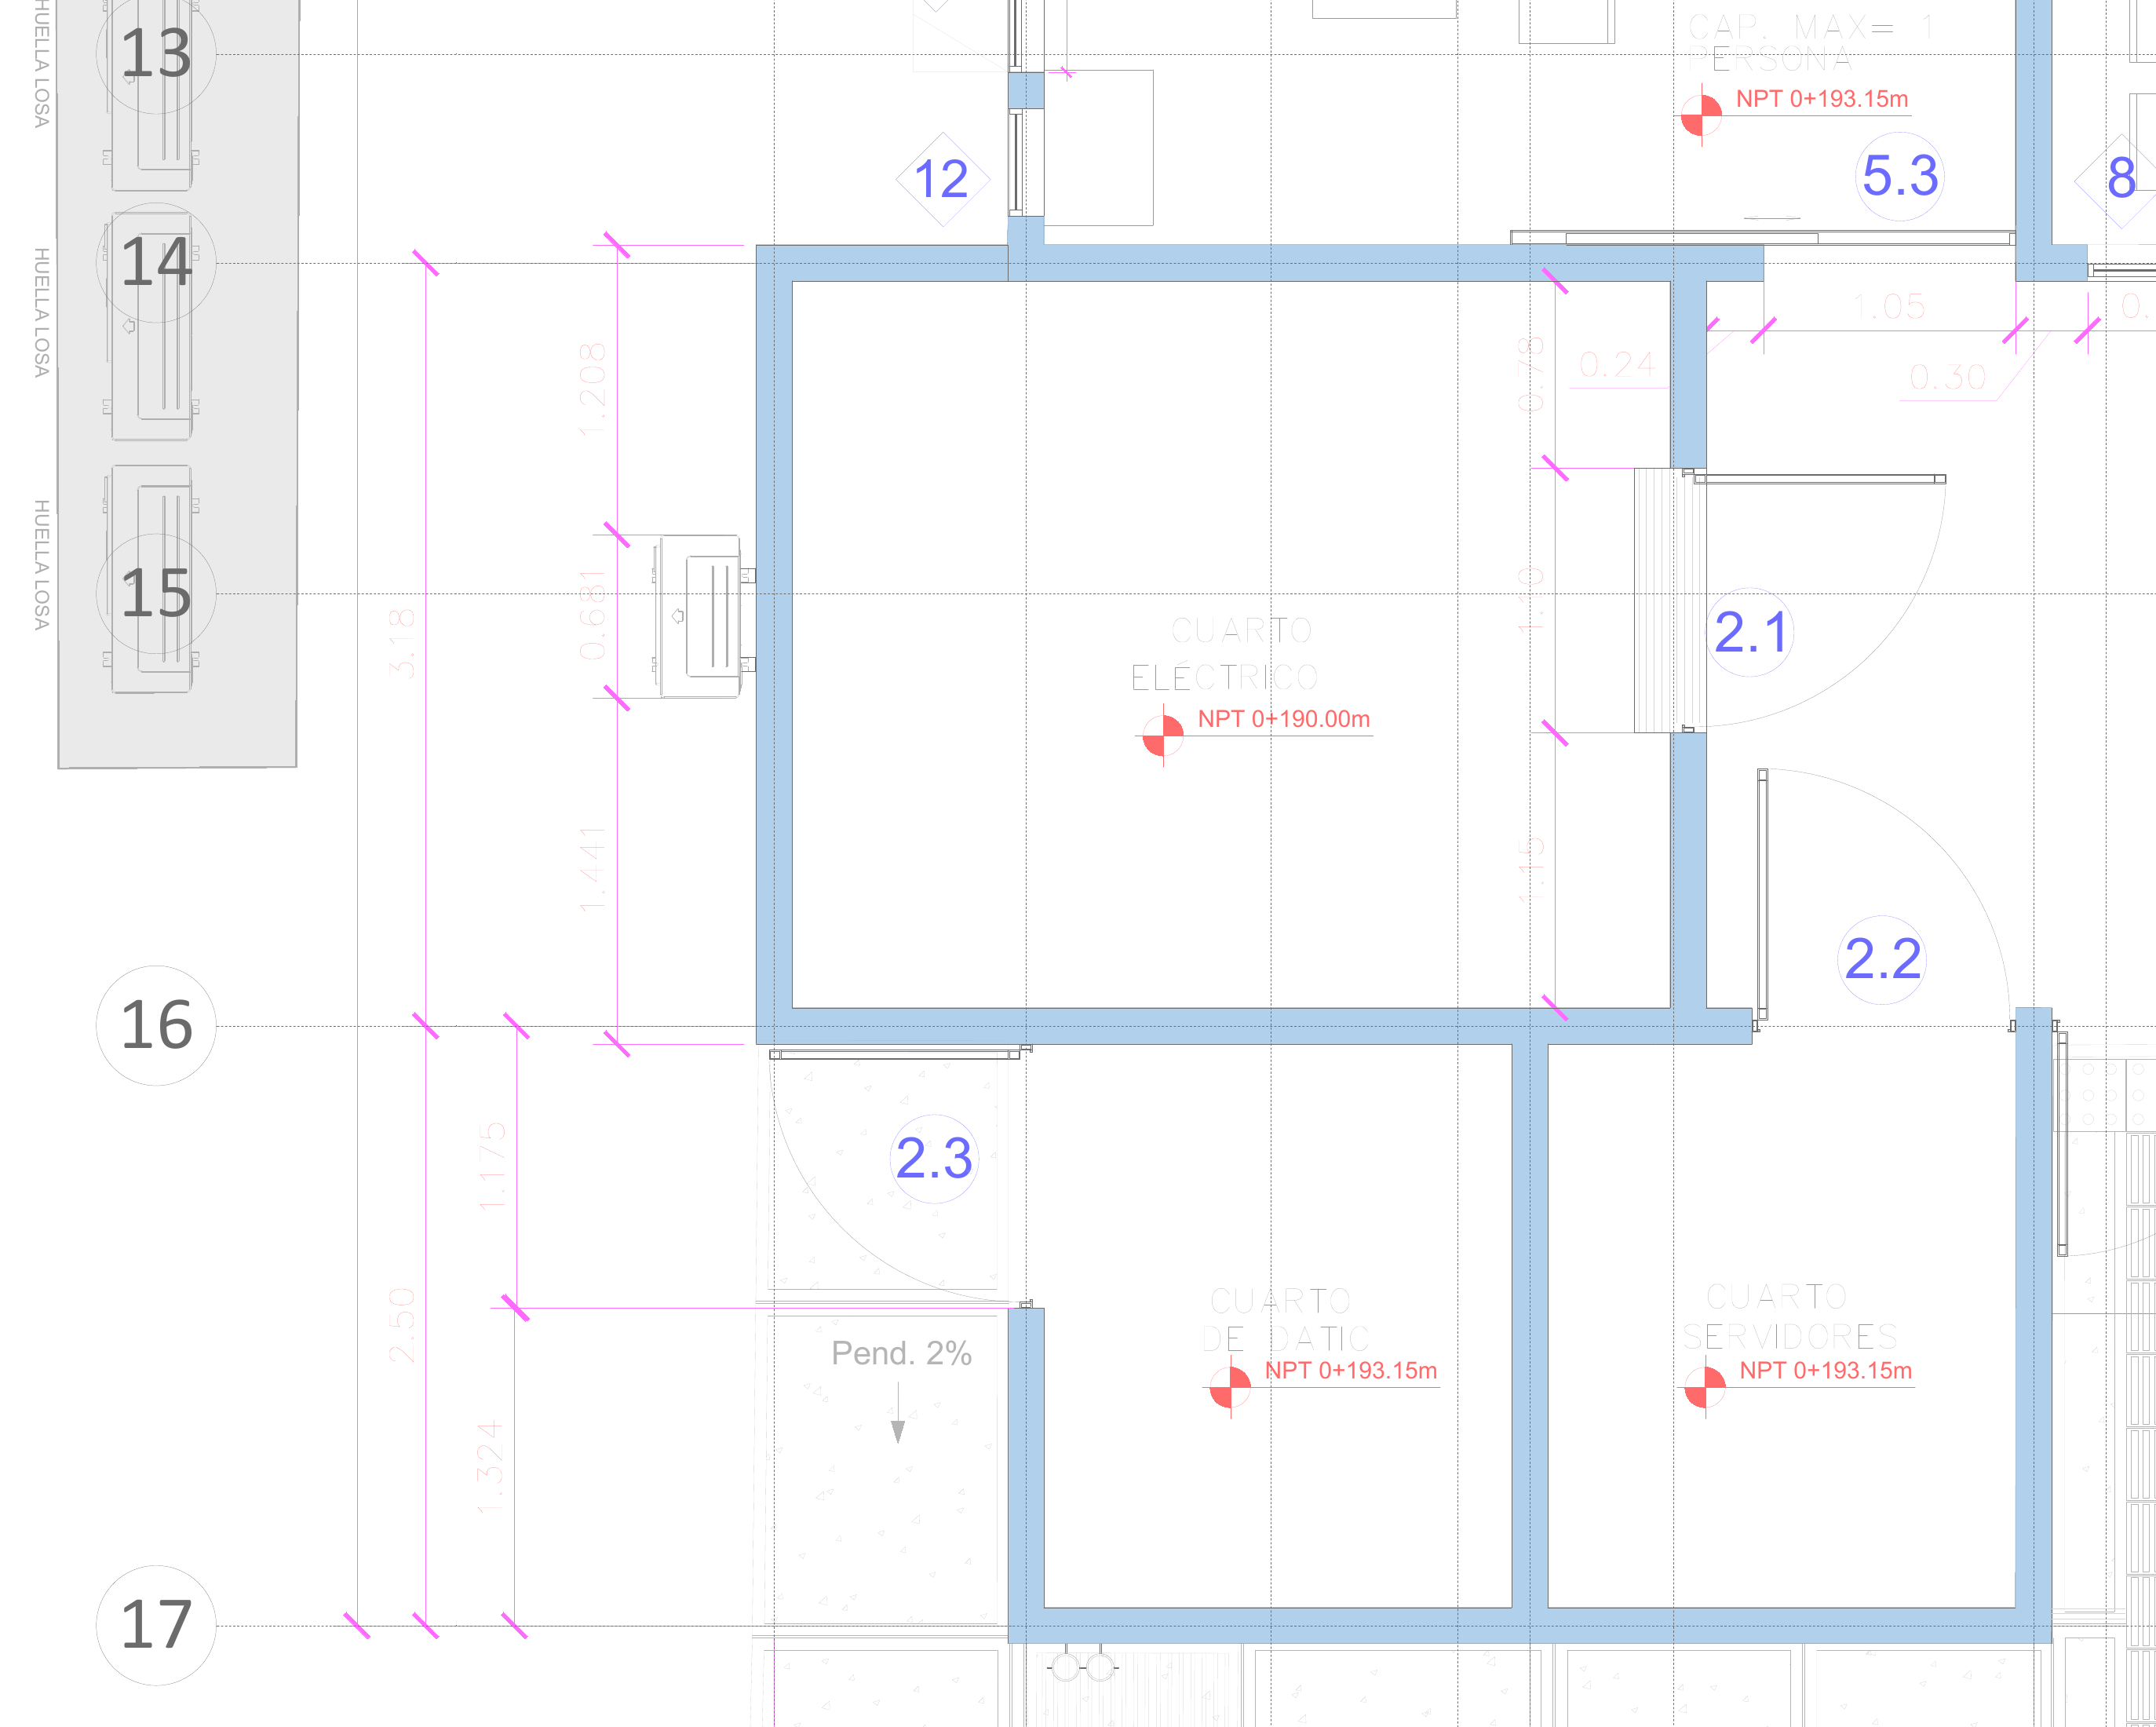
\includegraphics[width=180mm]{fv02_base.png}};
\draw[line width=0.4pt] (-3.0,12.6) rectangle (6.0,19.8);
\draw[draw=exist,fill=exist!25,line width=0.4pt] (0.31,13.90) rectangle (0.56,14.35);
\node[anchor=west,font=\fontsize{4.8}{5}\selectfont,text=exist!80!black,inner sep=0.5pt] at (0.62,14.12) {TM-UPS};
\draw[draw=exist,fill=exist!25,line width=0.4pt] (0.31,14.42) rectangle (0.61,15.07);
\node[anchor=west,font=\fontsize{4.8}{5}\selectfont,text=exist!80!black,inner sep=0.5pt] at (0.64,14.96) {TS-01};
\draw[draw=exist,fill=exist!25,line width=0.4pt] (0.31,15.12) rectangle (0.56,15.78);
\node[anchor=west,font=\fontsize{4.8}{5}\selectfont,text=exist!80!black,inner sep=0.5pt] at (0.62,15.45) {ATS (TA-GR)};
\draw[draw=exist,fill=exist!25,line width=0.4pt] (0.31,15.85) rectangle (0.56,16.60);
\node[anchor=west,font=\fontsize{4.8}{5}\selectfont,text=exist!80!black,inner sep=0.5pt] at (0.62,16.22) {TP};
\draw[draw=exist,fill=exist!25,line width=0.4pt] (0.75,16.55) rectangle (1.25,16.78);
\node[anchor=south,font=\fontsize{4.8}{5}\selectfont,text=exist!80!black,inner sep=0.5pt] at (1.00,16.40) {TN1};
\draw[draw=exist,fill=exist!25,line width=0.4pt] (1.35,16.55) rectangle (1.85,16.78);
\node[anchor=south,font=\fontsize{4.8}{5}\selectfont,text=exist!80!black,inner sep=0.5pt] at (1.60,16.40) {TI1};
\draw[draw=exist,fill=exist!25,line width=0.4pt] (1.95,16.55) rectangle (2.45,16.78);
\node[anchor=south,font=\fontsize{4.8}{5}\selectfont,text=exist!80!black,inner sep=0.5pt] at (2.20,16.40) {TRU1};
\draw[draw=exist,fill=exist!25,line width=0.4pt] (2.55,16.55) rectangle (3.05,16.78);
\node[anchor=south,font=\fontsize{4.8}{5}\selectfont,text=exist!80!black,inner sep=0.5pt] at (2.80,16.40) {TD1};
\draw[draw=exist,fill=exist!25,line width=0.4pt] (3.40,13.80) rectangle (3.95,14.20);
\node[anchor=north,font=\fontsize{4.8}{5}\selectfont,text=exist!80!black,inner sep=0.5pt] at (3.67,14.30) {PCA/PDI};
\draw[exist,line width=0.4pt,pattern=crosshatch,pattern color=exist!40] (1.05,13.80) rectangle (2.30,14.95);
\draw[draw=exist,fill=exist!25,line width=0.4pt] (1.40,14.05) rectangle (1.95,14.70);
\node[font=\fontsize{4.8}{5}\selectfont,text=exist!80!black] at (1.675,14.375) {UPS};
\draw[exist,fill=white,line width=0.4pt] (-0.40,14.85) rectangle (0.17,15.47); \draw[exist,line width=0.3pt] (-0.115,15.16) circle (0.18);
\draw[draw=inv1,fill=inv1!25,line width=0.6pt] (-0.13,15.65) rectangle (0.17,15.97);
\draw[draw=inv2,fill=inv2!25,line width=0.6pt] (-0.13,16.25) rectangle (0.17,16.57);
\draw[draw=nuevo,fill=nuevo!18,line width=0.6pt] (0.02,13.82) rectangle (0.17,14.27);
\draw[draw=nuevo,fill=nuevo!18,line width=0.6pt] (-0.05,14.37) rectangle (0.17,14.75);
\draw[draw=nuevo,fill=nuevo!18,line width=0.6pt,pattern=north east lines,pattern color=nuevo] (0.31,14.45) rectangle (0.51,15.00);
\draw[nuevo,line width=0.35pt,dash pattern=on 2pt off 1pt] (-1.03,15.55) rectangle (-0.13,16.67);
\draw[nuevo,line width=0.35pt,dash pattern=on 2pt off 1pt] (-0.95,13.75) rectangle (-0.05,14.80);
\node[font=\fontsize{4.6}{5}\selectfont,text=nuevo,rotate=90] at (-0.85,16.11) {0,90 m};
\node[font=\fontsize{4.6}{5}\selectfont,text=nuevo,rotate=90] at (-0.80,14.28) {0,90 m};
\filldraw[dc,draw=black,line width=0.3pt] (0.02,16.11) circle (0.07);
\draw[dc,line width=1.1pt] (0.02,16.11) -- (0.02,15.97); \draw[dc,line width=1.1pt] (0.02,16.11) -- (0.02,16.25);
\draw[black,line width=0.8pt] (0.10,16.57) -- (0.10,16.70) -- (0.24,16.70);
\draw[black,line width=0.9pt,dash pattern=on 3pt off 1pt] (0.12,15.65) -- (0.12,14.27);
\draw[nuevo,line width=1.0pt] (0.17,14.56) -- (0.31,14.56);
\draw[violet,line width=0.6pt,dash pattern=on 2pt off 1pt] (0.17,16.45) -- (0.40,16.45) -- (0.40,16.95) -- (1.80,16.95) -- (1.80,17.55);
\node[draw=violet,font=\fontsize{4.6}{5}\selectfont,text=violet,fill=white,inner sep=1pt] at (1.80,17.75) {RACK};
\draw[inv1,line width=0.3pt] (-0.13,15.81) -- (-1.35,15.30);
\node[anchor=east,font=\fontsize{5.6}{6.4}\selectfont\bfseries,text=inv1,fill=white,inner sep=0.8pt,align=right] at (-1.35,15.30) {INV-1};
\draw[inv2,line width=0.3pt] (-0.13,16.41) -- (-1.35,16.95);
\node[anchor=east,font=\fontsize{5.6}{6.4}\selectfont\bfseries,text=inv2,fill=white,inner sep=0.8pt,align=right] at (-1.35,16.95) {INV-2};
\draw[dc,line width=0.3pt] (0.02,16.11) -- (-1.35,16.30);
\node[anchor=east,font=\fontsize{5.6}{6.4}\selectfont\bfseries,text=dc,fill=white,inner sep=0.8pt,align=right] at (-1.35,16.30) {BJ-DC};
\draw[nuevo,line width=0.3pt] (-0.05,14.56) -- (-1.25,14.95);
\node[anchor=east,font=\fontsize{5.6}{6.4}\selectfont\bfseries,text=nuevo,fill=white,inner sep=0.8pt,align=right] at (-1.25,14.95) {IFV};
\draw[nuevo,line width=0.3pt] (0.02,14.05) -- (-1.25,13.40);
\node[anchor=east,font=\fontsize{5.6}{6.4}\selectfont\bfseries,text=nuevo,fill=white,inner sep=0.8pt,align=right] at (-1.25,13.40) {TFV};
\draw[nuevo,line width=0.3pt] (0.41,14.72) -- (1.15,13.25);
\node[anchor=east,font=\fontsize{5.6}{6.4}\selectfont\bfseries,text=nuevo,fill=white,inner sep=0.8pt,align=right] at (1.15,13.25) {CD-FV};
\node[anchor=north,font=\fontsize{4.6}{5}\selectfont,text=exist!80!black,fill=white,inner sep=0.6pt] at (-0.12,15.50) {UC (exist.)};
\draw[black,line width=0.5pt,-{Latex[length=1.6mm]}] (-1.9,13.65) -- (-1.9,13.95); \draw[black,line width=0.5pt,-{Latex[length=1.6mm]}] (-1.9,16.95) -- (-1.9,16.65);
\draw[black,line width=0.3pt,dash pattern=on 4pt off 1pt on 1pt off 1pt] (-1.9,13.65) -- (-1.9,16.95);
\node[font=\fontsize{5.5}{6}\selectfont\bfseries,fill=white,inner sep=0.6pt] at (-2.15,13.55) {E1};
\node[font=\fontsize{5.5}{6}\selectfont\bfseries,fill=white,inner sep=0.6pt] at (-2.15,17.05) {E1};
\node[font=\fontsize{5.5}{6}\selectfont\bfseries,fill=white,inner sep=0.8pt] at (-2.1,18.6) {EXTERIOR (fachada sur)};
\begin{scope}[shift={(4.9,18.9)}]
\draw[line width=0.4pt] (0,0) circle (0.42);
\fill[black] (0.55,0) -- (-0.25,0.18) -- (-0.10,0) -- (-0.25,-0.18) -- cycle;
\node[font=\fontsize{6}{7}\selectfont\bfseries] at (0.82,0) {N};
\end{scope}
\end{scope}
\node[anchor=north west,font=\fontsize{9}{11}\selectfont\bfseries] at (20,135.5) {PLANTA PARCIAL NIVEL 1 -- FACHADA SUR (EJE A) Y CUARTO ELÉCTRICO};
\node[anchor=north west,font=\fontsize{6.5}{7.5}\selectfont] at (20,131) {Escala 1:50 (A3). Base: planta A01 nivel 1 (as-built). Equipos existentes transcritos de E01 (posición aproximada).};
\draw[fill=exist!8,draw=exist,line width=0.5pt] (31.25,27.00) rectangle (111.25,98.25);
\draw[line width=0.8pt] (25.00,27.00) -- (116.25,27.00);
\fill[pattern=north east lines,pattern color=exist] (25.00,24.00) rectangle (116.25,27.00);
\node[font=\fontsize{5.2}{6}\selectfont,anchor=north] at (102.50,22.50) {Rasante exterior $\approx$ 192,3 (E01)};
\node[font=\fontsize{5.2}{6}\selectfont,anchor=west] at (37.50,94.50) {Muro eje A (continúa hasta el alero, $\approx$ 7,5 m)};
\draw[draw=exist,fill=white,line width=0.4pt,dash pattern=on 2pt off 1pt] (60.00,34.50) rectangle (75.50,50.75);
\node[font=\fontsize{5.2}{6}\selectfont,text=exist] at (67.75,42.50) {UC exist.};
\draw[draw=nuevo,fill=nuevo!18,line width=0.6pt] (34.25,54.50) rectangle (45.50,70.75);
\node[font=\fontsize{5.2}{6}\selectfont,text=nuevo] at (39.88,64.00) {\textbf{TFV}};
\draw[draw=nuevo,fill=nuevo!18,line width=0.6pt] (48.00,53.25) rectangle (57.50,68.25);
\node[font=\fontsize{5.2}{6}\selectfont,text=nuevo] at (52.75,62.00) {\textbf{IFV}};
\draw[nuevo,line width=1.2pt] (56.25,59.50) -- (59.50,59.50);
\draw[draw=inv1,fill=inv1!25,line width=0.6pt] (80.00,49.50) rectangle (88.00,69.75);
\node[font=\fontsize{5.2}{6}\selectfont,text=inv1,rotate=90] at (84.00,59.50) {\textbf{INV-1}};
\draw[draw=inv2,fill=inv2!25,line width=0.6pt] (95.00,49.50) rectangle (103.00,69.75);
\node[font=\fontsize{5.2}{6}\selectfont,text=inv2,rotate=90] at (99.00,59.50) {\textbf{INV-2}};
\draw[dc,line width=1.3pt] (90.25,98.25) -- (90.25,75.75);
\draw[dc,line width=1.3pt] (92.25,98.25) -- (92.25,75.75);
\draw[dc,line width=1.3pt] (90.25,75.75) -- (84.00,75.75) -- (84.00,69.75);
\draw[dc,line width=1.3pt] (92.25,75.75) -- (99.00,75.75) -- (99.00,69.75);
\node[anchor=south,font=\fontsize{5.2}{6}\selectfont,text=dc] at (91.25,98.75) {2 EMT 3/4'' DC desde BJ-DC (FV-01)};
\draw[black,line width=1.0pt] (84.00,49.50) -- (84.00,32.00) -- (41.25,32.00) -- (41.25,54.50);
\draw[black,line width=1.0pt] (99.00,49.50) -- (99.00,32.00) -- (84.00,32.00);
\node[font=\fontsize{5.2}{6}\selectfont,anchor=west] at (42.25,29.50) {EMT AC a h = 0,20 m};
\draw[black,line width=1.0pt] (45.50,59.50) -- (48.00,59.50);
\draw[nuevo,line width=1.0pt] (52.75,53.25) -- (52.75,40.75);
\draw[nuevo,line width=0.4pt] (52.75,40.75) circle (1.1);
\node[font=\fontsize{5.2}{6}\selectfont,anchor=east,text=nuevo,align=right] at (51.75,46.50) {Pasamuro\\a CD-FV};
\draw[nuevo,line width=0.3pt,dash pattern=on 3pt off 1.5pt] (31.25,77.00) -- (111.25,77.00);
\node[anchor=south west,font=\fontsize{5}{6}\selectfont,text=nuevo] at (32.25,77.00) {Máx. altura de maniobra 2,00 m (NEC 240.24(A), 404.8)};
\draw[line width=0.25pt,{Bar[width=1.4mm]Latex[length=1mm]}-{Latex[length=1mm]Bar[width=1.4mm]}] (107.50,27.00) -- (107.50,49.50);
\node[font=\fontsize{5}{6}\selectfont,rotate=90,fill=white,inner sep=0.5pt] at (105.70,38.25) {0,90};
\draw[line width=0.25pt,{Bar[width=1.4mm]Latex[length=1mm]}-{Latex[length=1mm]Bar[width=1.4mm]}] (107.50,49.50) -- (107.50,69.75);
\node[font=\fontsize{5}{6}\selectfont,rotate=90,fill=white,inner sep=0.5pt] at (105.70,59.62) {0,81};
\draw[line width=0.25pt,{Bar[width=1.4mm]Latex[length=1mm]}-{Latex[length=1mm]Bar[width=1.4mm]}] (28.75,27.00) -- (28.75,77.00);
\node[font=\fontsize{5}{6}\selectfont,rotate=90,fill=white,inner sep=0.5pt] at (26.95,52.00) {2,00};
\draw[line width=0.25pt,{Bar[width=1.4mm]Latex[length=1mm]}-{Latex[length=1mm]Bar[width=1.4mm]}] (31.25,13.25) -- (111.25,13.25);
\node[font=\fontsize{5}{6}\selectfont,fill=white,inner sep=0.5pt] at (71.25,13.25) {3,18 m (ejes 14--16)};
\draw[exist,line width=0.2pt,dash pattern=on 3pt off 1pt on 0.6pt off 1pt] (31.75,99.25) -- (31.75,104.25);
\node[circle,draw=exist,minimum size=3.6mm,inner sep=0pt,font=\fontsize{5}{5}\selectfont] at (31.75,106.25) {14};
\draw[exist,line width=0.2pt,dash pattern=on 3pt off 1pt on 0.6pt off 1pt] (66.25,99.25) -- (66.25,104.25);
\node[circle,draw=exist,minimum size=3.6mm,inner sep=0pt,font=\fontsize{5}{5}\selectfont] at (66.25,106.25) {15};
\draw[exist,line width=0.2pt,dash pattern=on 3pt off 1pt on 0.6pt off 1pt] (111.25,99.25) -- (111.25,104.25);
\node[circle,draw=exist,minimum size=3.6mm,inner sep=0pt,font=\fontsize{5}{5}\selectfont] at (111.25,106.25) {16};
\node[anchor=north west,font=\fontsize{9}{11}\selectfont\bfseries] at (20,122) {ELEVACIÓN E1 -- FACHADA SUR (vista desde el exterior)};
\node[anchor=north west,font=\fontsize{6.5}{7.5}\selectfont,align=left] at (20,117.5) {Escala 1:40. Alturas desde la rasante exterior. Cotas en metros.};
\node[anchor=north west,font=\fontsize{5.3}{6.4}\selectfont] at (128,108) {%
\setlength{\tabcolsep}{2pt}\begin{tabular}{@{}lll@{}}
\textbf{ID} & \textbf{Equipo / modelo} & \textbf{Montaje}\\\hline
INV-1/2 & SolarEdge SE10KUS, 208Y/120 V, NEMA 3R & h 0,90--1,71 m\\
 & 808 $\times$ 317 $\times$ 300 mm, 35,5 kg & exterior\\
TFV & Square D NQ 3$\phi$ 4h, barras 100 A, & h 1,10--1,75 m\\
 & 2 $\times$ QOB335 + SPD tipo 2, gab. NEMA 3R & exterior\\
IFV & Square D HU363RB, 100 A, 600 V, sin & h 1,05--1,65 m\\
 & fusibles, corte visible, con candado & exterior\\
CD-FV & Bloque UL 1953 + interruptor 70 A/3P & muro interior\\
 & (PowerPact HDL36070) + TC del medidor & junto a TS-01\\
IS-TS01 & Interruptor 400 A/3P PowerPact LAL36400, & muro interior,\\
 & gab. NEMA 1, a $\le$ 3 m de TS-01 & junto a CD-FV\\
BJ-DC & 2 $\times$ EMT 3/4'' con PV Wire \#10 & fachada\\\hline
\end{tabular}};
\node[anchor=north west,font=\fontsize{9}{11}\selectfont\bfseries] at (252,284) {LEYENDA};
\begin{scope}[shift={(252,276)}]
\filldraw[fill=inv1!25,draw=inv1,line width=0.6pt] (0,0) rectangle (6,-3.5);
\node[anchor=west,font=\fontsize{6}{7}\selectfont] at (8,-1.75) {Inversor INV-1 / INV-2 (SolarEdge SE10KUS), nuevo};
\filldraw[fill=nuevo!18,draw=nuevo,line width=0.6pt] (0,-5.5) rectangle (6,-9);
\node[anchor=west,font=\fontsize{6}{7}\selectfont] at (8,-7.25) {Tablero / desconectador / derivación nuevo (TFV, IFV, CD-FV)};
\filldraw[fill=exist!25,draw=exist,line width=0.4pt] (0,-11) rectangle (6,-14.5);
\node[anchor=west,font=\fontsize{6}{7}\selectfont] at (8,-12.75) {Equipo existente (E01, posición aproximada)};
\draw[nuevo,line width=0.35pt,dash pattern=on 2pt off 1pt] (0,-16.5) rectangle (6,-20);
\node[anchor=west,font=\fontsize{6}{7}\selectfont] at (8,-18.25) {Espacio de trabajo libre NEC 110.26 (0,90 m de profundidad)};
\draw[dc,line width=1.3pt] (0,-23) -- (6,-23);
\node[anchor=west,font=\fontsize{6}{7}\selectfont] at (8,-23) {Canalización DC (EMT), desde la cubierta};
\draw[black,line width=1.0pt] (0,-27) -- (6,-27);
\node[anchor=west,font=\fontsize{6}{7}\selectfont] at (8,-27) {Canalización AC (EMT): C-AC1, C-AC2, C-AC3};
\draw[nuevo,line width=1.0pt] (0,-31) -- (6,-31);
\node[anchor=west,font=\fontsize{6}{7}\selectfont] at (8,-31) {Conexión IFV $\rightarrow$ CD-FV a través del muro};
\draw[violet,line width=0.6pt,dash pattern=on 2pt off 1pt] (0,-35) -- (6,-35);
\node[anchor=west,font=\fontsize{6}{7}\selectfont] at (8,-35) {Comunicación UTP Cat6 al rack de DATIC (monitoreo)};
\end{scope}
\node[anchor=north west,font=\fontsize{9}{11}\selectfont\bfseries] at (252,232) {EQUIPOS EXISTENTES (E01, E07)};
\node[anchor=north west,font=\fontsize{5.8}{7.2}\selectfont,align=left,text width=152mm] at (252,226) {%
\textbf{TS-01 (TX)} Square D EXN112T3H, 112,5 kVA, 480$\Delta$--208Y/120 V, Z = 3,57 \% \quad \textbf{ATS (TA-GR)} Kohler KSS-ACTC-0400S, 400 A\\
\textbf{TP} Square D HCP32688, barras 800 A, principal LA36400 400 A, 42 polos (2--12 libres) \quad \textbf{TM-UPS} Eaton, 100 A, doble tiro\\
\textbf{TN1, TI1, TRU1, TD1} tableros secundarios \quad \textbf{UPS} Ablerex 20 kVA \quad \textbf{UC} condensadora del cuarto eléctrico};
\node[anchor=north west,font=\fontsize{9}{11}\selectfont\bfseries] at (252,206) {NOTAS};
\node[anchor=north west,font=\fontsize{5.8}{7.2}\selectfont,align=left,text width=152mm] at (252,200) {%
1. Según E01, el muro interior del eje A del cuarto eléctrico ya está ocupado por TM-UPS, TS-01, ATS y TP. Por eso los inversores, el TFV y el IFV se instalan en la cara \textbf{exterior} del mismo muro (fachada sur), bajo el alero, en envolventes NEMA 3R.\\
2. Los circuitos DC nunca entran al edificio: bajan por la fachada (BJ-DC) directamente a los inversores (NEC 690.31).\\
3. A la salida de TS-01 se instala el interruptor secundario IS-TS01 (400 A/3P, a $\le$ 3 m, NEC 240.21(C)(2)); aguas abajo, la derivación al alimentador protegido IS-TS01 $\rightarrow$ ATS se hace dentro de CD-FV (bloque UL 1953) y termina, a menos de 3 m, en un interruptor de 70 A/3P (NEC 240.21(B)(1), 705.12(B)(2)). IS-TS01 se monta en el muro interior junto a CD-FV, con manija a $\le$ 2,00 m y el espacio de trabajo de NEC 110.26.\\
4. El IFV es el desconectador del sistema FV y el iniciador del apagado rápido. Es accesible desde el exterior para el ICE y Bomberos, tiene corte visible y se puede bloquear con candado (NEC 690.12(C), 690.13, 705.20).\\
5. Mantener 0,90 m de profundidad libre, 0,76 m de ancho y 2,00 m de altura frente a cada equipo (NEC 110.26). Ninguna manija de operación a más de 2,00 m.\\
6. El cuarto eléctrico está unos 2,3 m por debajo de la rasante exterior (NPT 0+190,00): el pasamuro, a h $\approx$ 0,55 m por fuera (bajo el IFV), llega a unos 2,85 m sobre el piso interior. C-AC4 baja en EMT por el muro interior hasta CD-FV, cuya manija queda a 1,70 m del piso del cuarto ($\le$ 2,00 m, NEC 240.24(A)). Pasamuro sellado con material cortafuego y sello hidráulico exterior.\\
7. La posición de la condensadora existente (UC) y de los equipos interiores se transcribe de E01 y del registro fotográfico del 5/10/2026; los equipos FV quedan a los costados de la UC y no obstruyen su descarga de aire ni su acceso de mantenimiento.\\
8. Generador: se adopta el dato de E07 (Kohler J100U-IV, 100 kW); E01 lo rotula como GR-01 de 55 kVA. No afecta la conexión FV, que queda del lado normal del ATS.};
\cajetin{FV-02}{Ubicación de inversores, tableros y desconectadores:}{planta parcial nivel 1 y elevación de fachada sur}{1:50 / 1:40}{3 de 5}
\end{tikzpicture}
\end{document}